\chapter{Workflow}
\label{workflow}

This chapter presents the features available for ProVANT Simulator's operation through the graphical interface, such as:

\begin{itemize}
\setlength{\itemsep}{1pt}
\setlength{\parskip}{0pt}
\setlength{\parsep}{0pt}
\item Scenario selection
\item UAV model selection
\item Scenario configuration
\item UAV settings
\item Simulation startup
\end{itemize}
 
\section{How to start the simulation environment}

Once the installation process has been gone through successfully as described in the previous chapter, the development of controllers in the simulation enviromnent can begin. To start the GUI, open a new terminal and type the following command:

\begin{bashcode}
 provant_gui
\end{bashcode}

The graphical interface to access the simulator will then be started, and the main window will show up, as depicted in Figure \ref{1}.

\begin{figure*}[!ht]
	\centering
	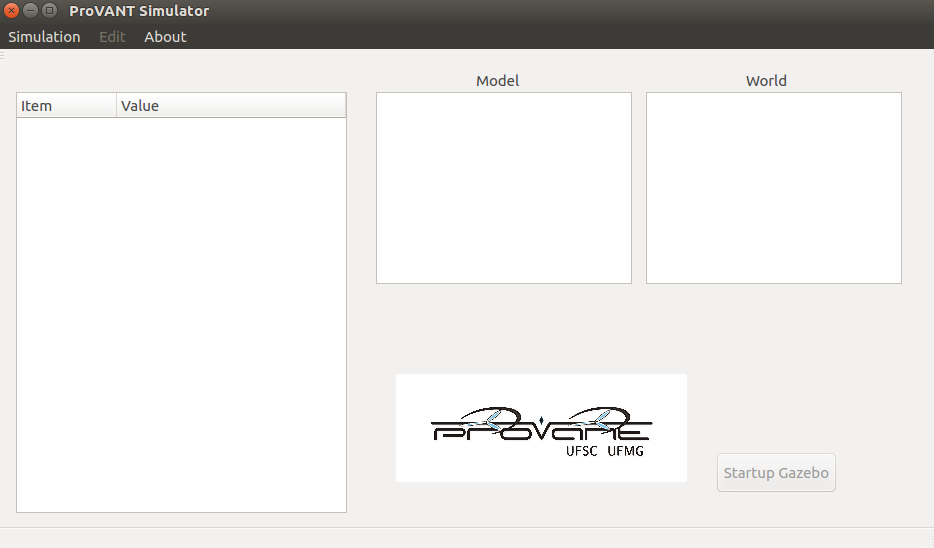
\includegraphics[width=0.8\columnwidth]{figuras/1.png}
	\caption{Main window}
	\label{1}
\end{figure*}

\section{Scenario selection}

Once the simulator's GUI has been started, the user must select a simulation scenario. That can be done in two different ways, through the option \textit{Simulation}, present in the GUI's top menu, as shown in figure \ref{2}:

\begin{figure*}[!ht]
	\centering
	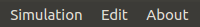
\includegraphics[width=100pt]{figuras/2.png}
	\caption{Top menu}
	\label{2}
\end{figure*}

\begin{itemize}
	\item[(i)] By clicking \textit{New}, a template scenario with extension \texttt{.tpl} can be opened.

	A template scenario is a scenario configuration that serves as template for the criation of other scenarios. It cannot be edited, needs the inclusion of a UAV model an must be saved before the simulation with format \texttt{.world}.
	 
	\item[(ii)] By clicking \textit{Open}, an existing sncenario (with extension \texttt{.world}) can be opened.
\end{itemize}

Menu \textit{Simulation} also allows to save a scenario with another name under the \texttt{.world} extension, by clicking \textit{Save}, and to end the simulation environment, by clicking \textit{Exit}.

\section{UAV selection}

Through option \textit{Edit} in the top menu, the UAV model to be used in the simulation can be selected. Note: in this version of the simulation environment, only a single UAV can be included in a given simulation instance.

\section{Simulation settings window}

After choosing the UAV and the simulation scenario, an illustrative image of the scenario will appear in the GUI. Thus, it is possible to verify if it was selected correctly, as shown in Figure \ref{tela_inicial.jpg}, through item 3.

\begin{figure*}[!ht]
	\centering
	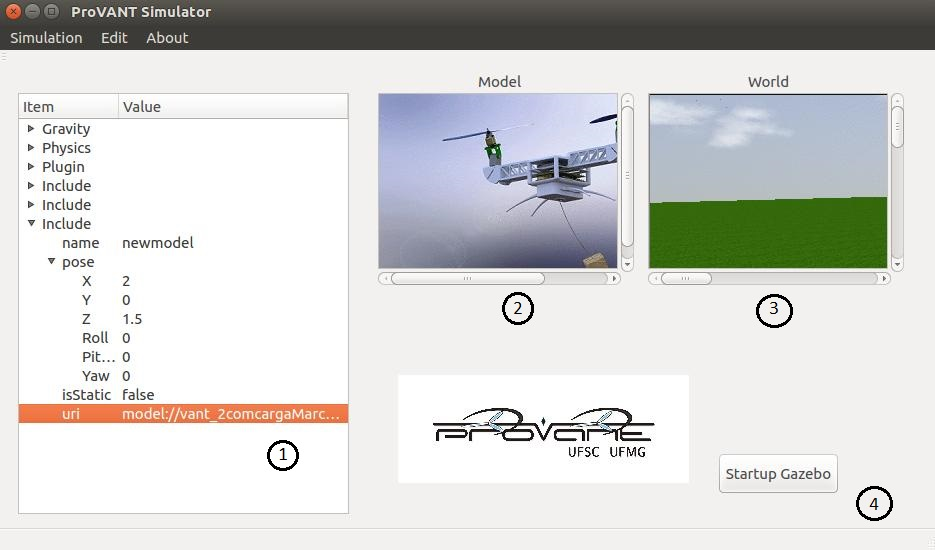
\includegraphics[width=500pt]{figuras/tela_inicial.jpg}
	\caption{Simulation settings window}
	\label{tela_inicial.jpg}
\end{figure*}

In this same window, item 1 consists of a tree with information and settings for the UAV and the simulation scenario. Settings can be edited by double-clicing the desired field. The main fields of this tree are:

\begin{itemize}
	\item Gravity: gravity acceleration vector with respect to the world frame, in m/s$^2$;
	\item Physics: physics engine used to perform the simulation. The available options are:
	\begin{itemize}
		\setlength{\itemsep}{1pt}
		\setlength{\parskip}{0pt}
		\setlength{\parsep}{0pt}
		\item ode
		\item bullet
		\item dart
		\item simbody
	\end{itemize}
	\item name: Name of the UAV model in simulator Gazebo
	\item pose: Initial position and orientation (roll, pitch, yaw) of the UAV, in meters and radians, respectively.
\end{itemize}

\noindent By double-clicking tue \textit{uri} field, a new window will open. In this window it is possible to view and configure the model, controller, actuators and sensors. More details on this window will be presented in the next section. Item 4 allows the initialization of the simulation with the settings, model and scenario selected by the user in the GUI.

\section{Model, control strategy and instrumentation visualization and settings window}
\label{SecEstCtrl}

\begin{figure*}[!ht]
	\centering
	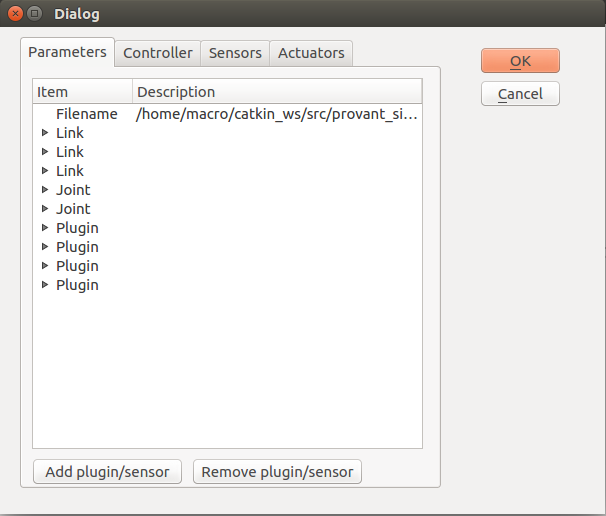
\includegraphics[width=250pt]{figuras/4.png}
	\caption{UAV model parameters visualization tab.}
	\label{4}
\end{figure*}

Figure \ref{5} shows tab \textit{Controller}. In this tab, it is possible to create a new contorl strategy, using item~2, select an existent one, through item 3, or compile it, item 4. The control strategi selected for use in the simulation is shown on item 1. More details on these items are fefscribed below.

\begin{figure*}[!ht]
	\centering
	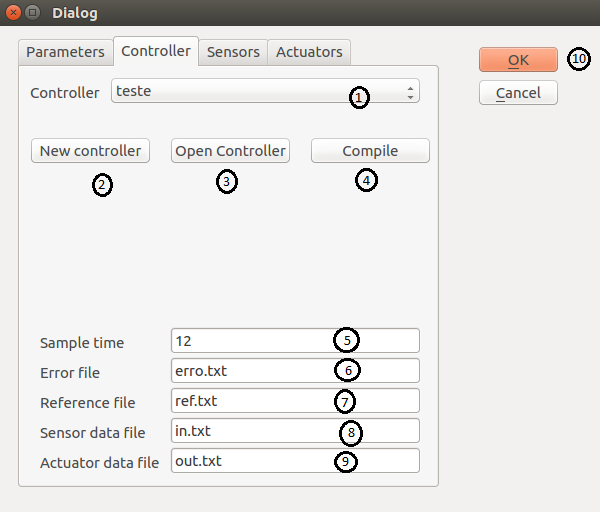
\includegraphics[width=250pt]{figuras/5_2.png}
	\caption{Control strategy selcection and configuration window.}
	\label{5}
\end{figure*}

\subsubsection{Creating a new control strategy}

To create a new control strategy, the button \textit{New controller} (item 2) must be clicked, and a new window will be shown (Figure \ref{9}). In this window, the user must insert the new control strategy's name (more details on the creation of a new control strategy are presented in Section \ref{controle}).

\begin{figure*}[!ht]
	\centering
	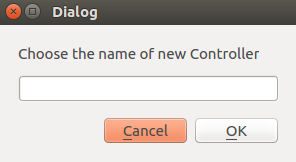
\includegraphics[width=100pt]{figuras/9.png}
	\caption{Creating a new control strategy.}
	\label{9}
\end{figure*}

\subsubsection{Modifying an existing control strategy}

To modify an ecisting control staregy, the user must select its name among several ones listed in the listing box (item 1) and click the button \textit{Open controller} (item 3). After choosing the strategy, the file manager Nautilus will be opened in the directory containing all the files and directories associated with the controller, as showin in Figure \ref{10}.

\begin{figure*}[!ht]
	\centering
	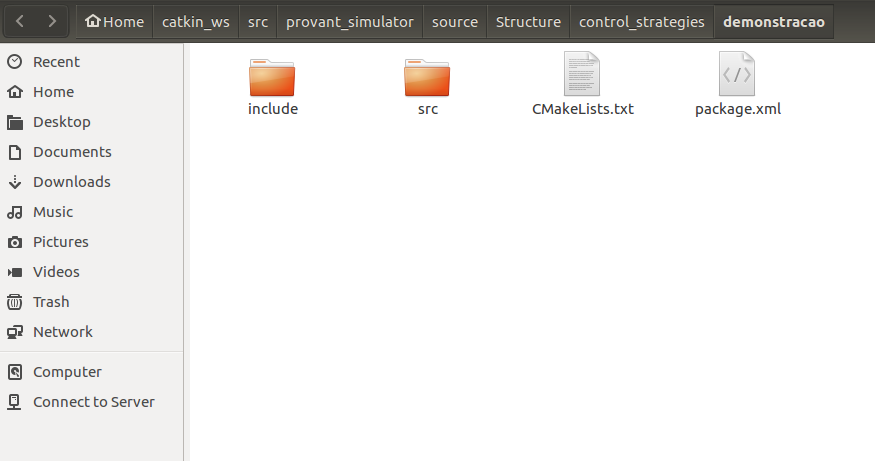
\includegraphics[width=300pt]{figuras/10.png}
	\caption{Directory containing all the files and folders associated to the control strategy to be modified.}
	\label{10}
\end{figure*}

\subsubsection{Compiling the contorller}

To compile the code associeted to the selected control strategy, the user must click the button \textit{Compile} (item 4). \textbf{This step must be executed whenever new modifications to the control strategy are made}. In case there are errors during compilation, the compiler's output log wil be shown in a text file on the text viewer gedit.

\subsubsection{Altering additional settings}

Tab \textit{Controller} also allows to setup other parameters related to the simulation. In field \textit{Sample time} (item 5), the sampling time in miliseconds can be configured. The remaining fields \textit{Error file} (item 6), \textit{Reference data file} (item 7), \textit{Sensor file} (item 8) amd \textit{Actuator data file} (item 9) determine the names of the text files where the values of the tracking error, desired path, sensor data and control signal will be logged, stored. These files can be loaded directly to MATLAB. They will available in the directory
\begin{bashcode}
$HOME/catkin_ws/srcProVANT-Simulator/source/Structure/Matlab
\end{bashcode}

\subsection{Selecting available instrumentation}
\label{sensoresatuadores}

Tabs \textit{Sensors} and \textit{Actuators} depicted in Figure \ref{6} list, respectively, the names of the sensors and actuators topics to which the controller will have access during simulation \textbf{in the presented order}. Those topics are configured during plugin configuration, and will be described in section \ref{plugins}. 

\begin{figure}
	\hfill
	\subfloat{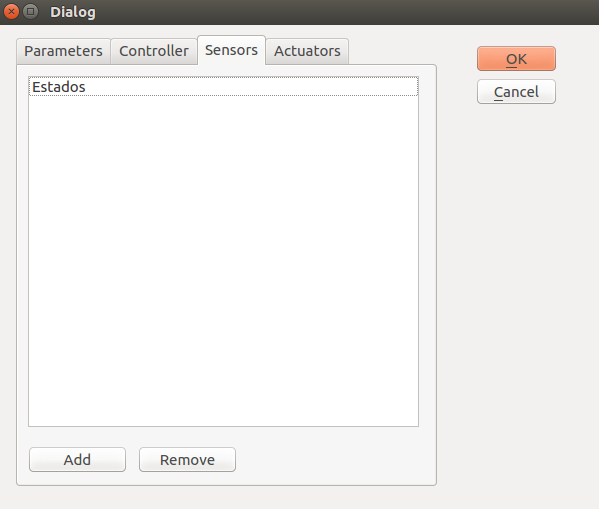
\includegraphics[width=230pt]{figuras/6.png}}
	\hfill
	\subfloat{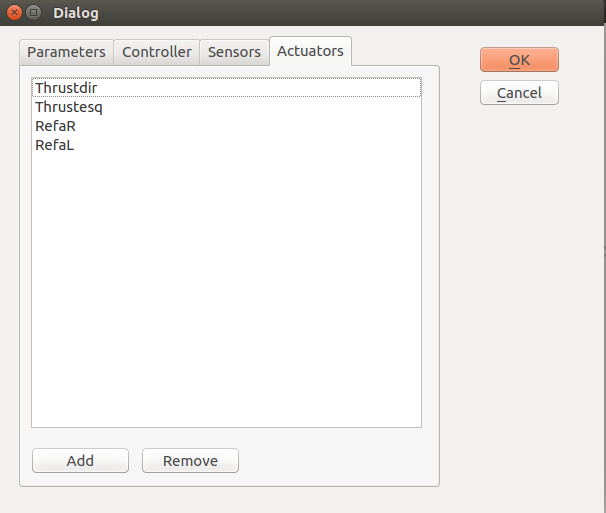
\includegraphics[width=230pt]{figuras/7.png}}
	\hfill
	\caption{Tabs for selecting the available instrumentation during simulation.}
	\label{6}
\end{figure}

\subsection{Starting the simulation}

After setting everything up, the user must press the button \textit{OK} (item 10). The simulation settings window (Figure \ref{tela_inicial.jpg}) will be shown again. The simulation can then be initialized with the selected UAV model, scenario, control straregy and instrumentation, by pressing the button \textit{Startup Gazebo} (item 4) of Figure \ref{tela_inicial.jpg}. The simulator Gazebo will be started, as shown in Figure \ref{12}. 

\begin{figure*}[!ht]
	\centering
	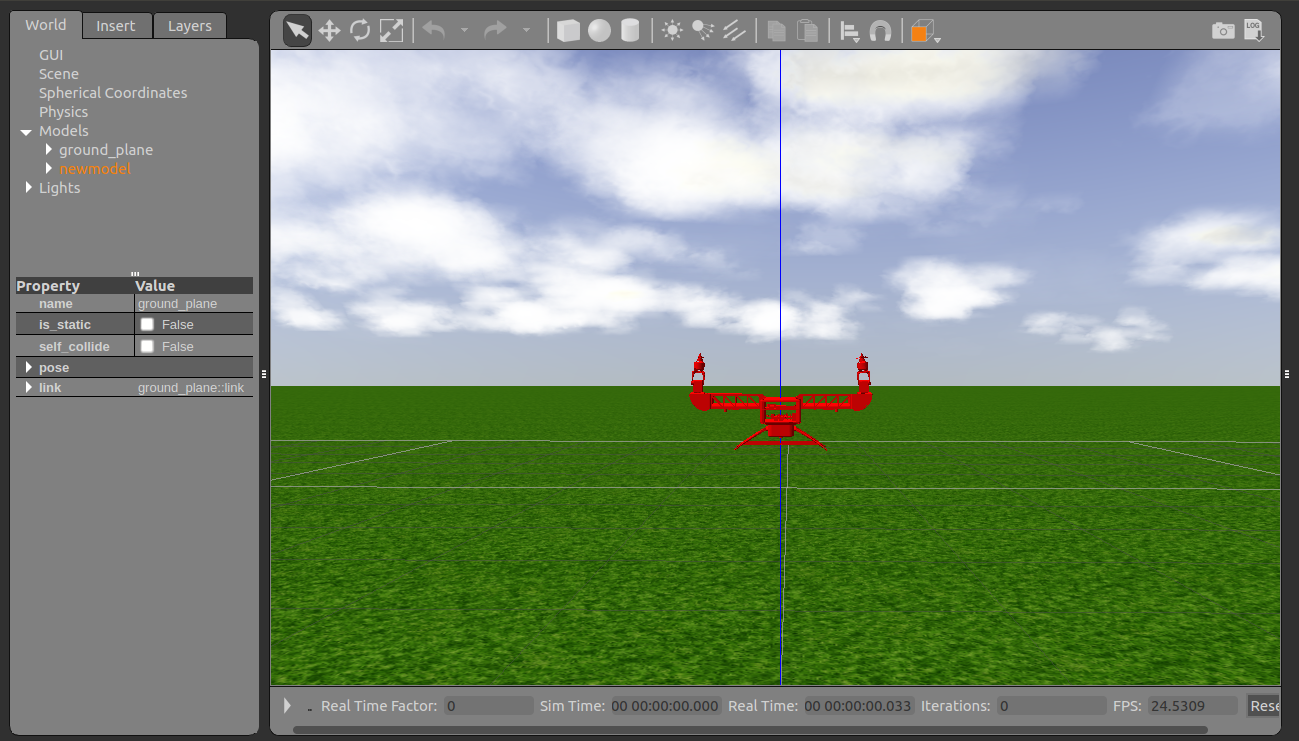
\includegraphics[width=400pt]{figuras/12.png}
	\caption{Gazebo's home window}
	\label{12}
\end{figure*}

To start the simulation, the user must press the button \textit{Step}. \textbf{Button \textit{Play} must not be used}.


%-----------------------------------------------------------------------


\section{Examples}


\subsection{UAV 4.0}

In order to execute the uav 4.0 simulation first the user should select in the user interface menu the option "Open" and then select the world file "vant4.world. Then, the user should in the same menu select the option "Edit" and then select the option that contains the model of the UAV 4.0. The UAV pose shall appear in the configuration window with the same pose as defined in the "vant4.world" file. In the case of the UAV 4.0 this pose is Position($0,4,0$) and Orientation($0,0,0$).



\begin{figure*}[!ht]
	\centering
	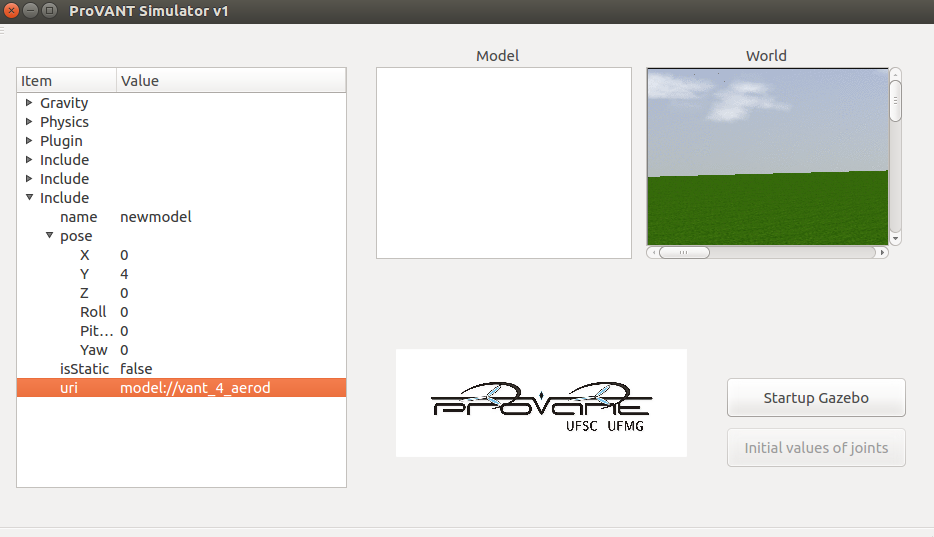
\includegraphics[width=250pt]{figuras/v4gui.png}
	\caption{Graphic Interface Window for UAV 4.0.}
	\label{v4gui}
\end{figure*}

By clicking twice the uri field, a configuration window for the model, controller, actuators and sensors will appear. In the tab "Controller" the control strategy "vant4Winf" should be selected and then compiled selecting the "Compile" button.


\begin{figure*}[!ht]
	\centering
	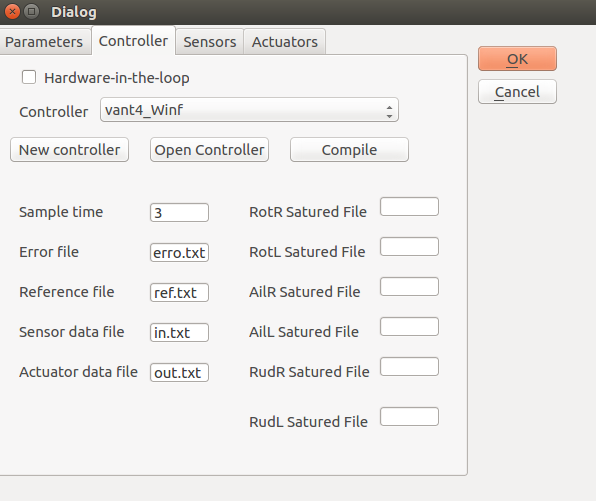
\includegraphics[width=150pt]{figuras/v4controllersetup.png}
	\caption{Configuration Screen for UAV 4.0 Control Strategy.}
	\label{v4controllersetup}
\end{figure*}

The simulation will then be configured and the user can select the option "Startup Gazebo" in the main window of the user interface to launch it. Finally, the user shoud select the Gazebo option "step" to effectively start the simulation.


\begin{figure*}[!ht]
	\centering
	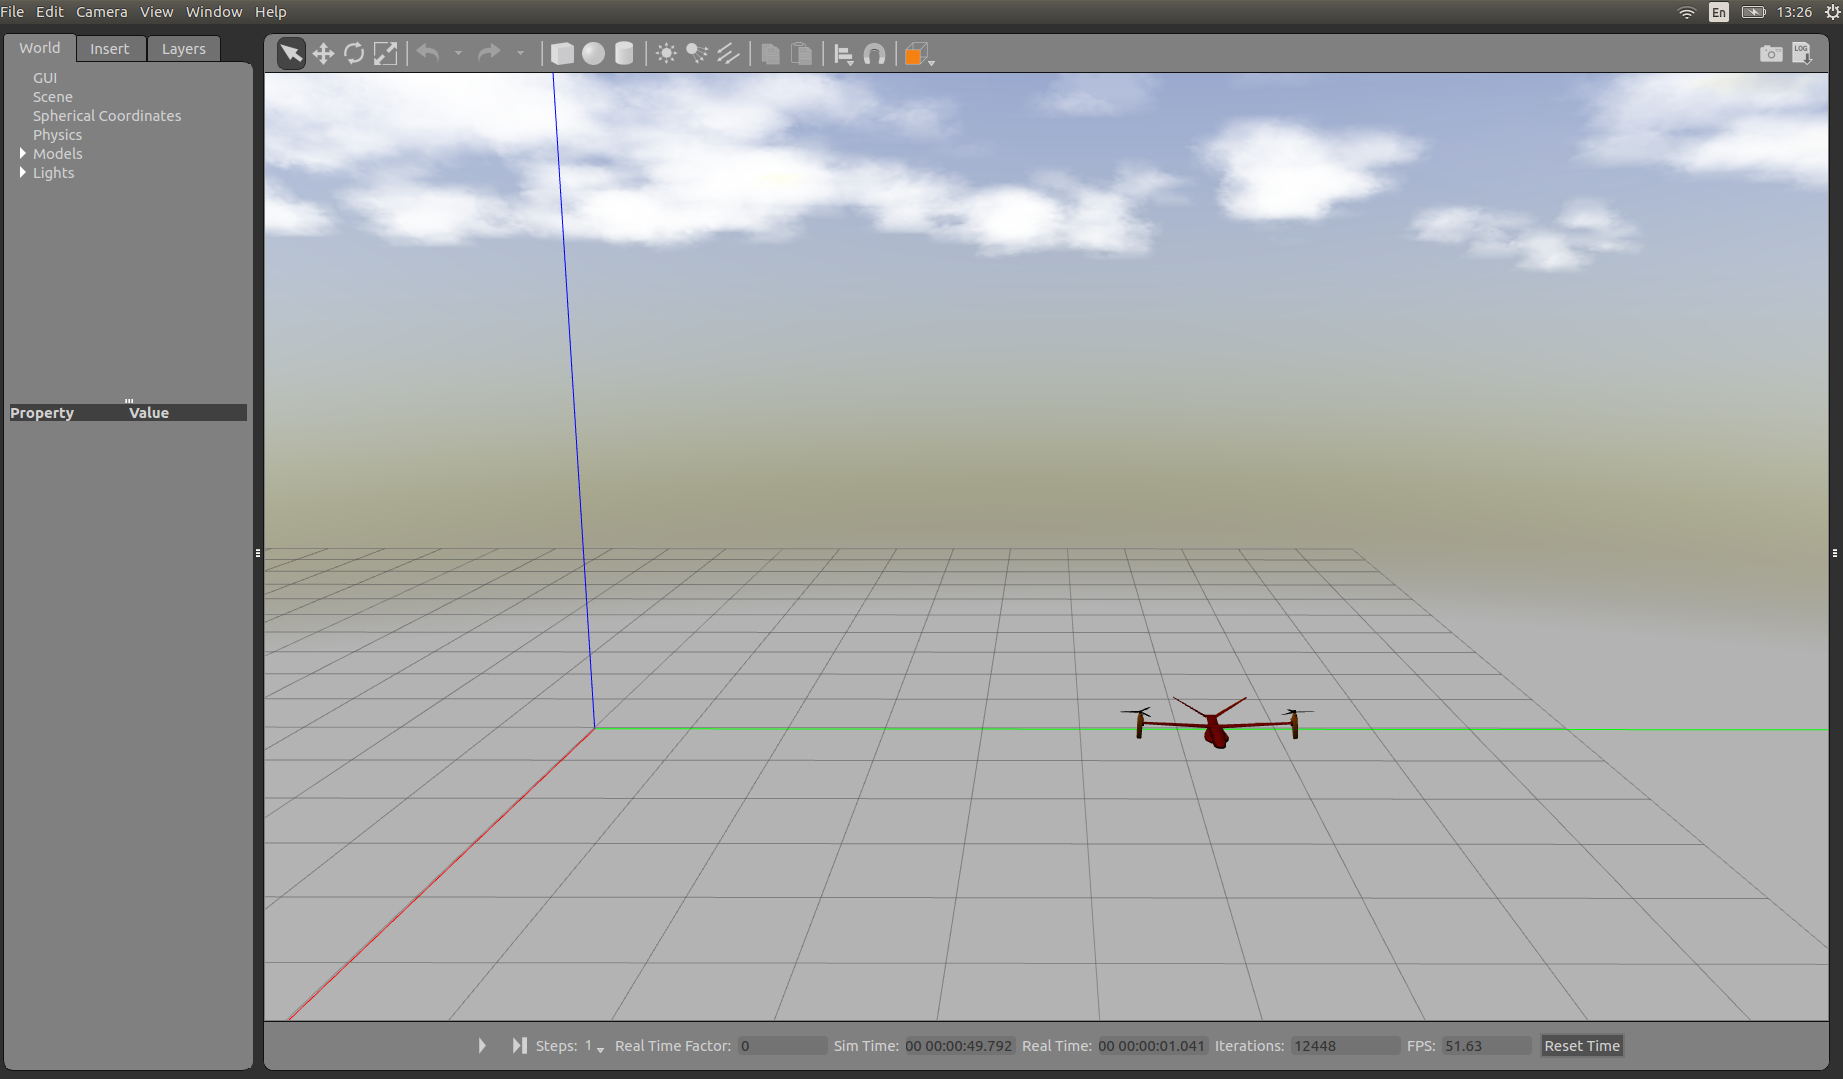
\includegraphics[width=350pt]{figuras/v4sim.png}
	\caption{UAV 4.0 Simulation.}
	\label{v4sim}
\end{figure*}

Using the "DataSaveTiltRotor" plugin, explained in the section \ref{plugins}, it's possible for the user to save the data of the forces applied by the thruster during the simulation, as well as the values of the deflexion of the rotors, ailerons and rudders. This values are saved in text files in the directory:
\begin{bashcode}
	$HOME/catkin_ws/src/ProVANT-Simulator/source/Structure/Matlab
	\end{bashcode}
	
	The values of the state error, desired trajectory, data from the sensors, and control signals can be found in text files in the Matlab directory.
	
	\subsection{UAV 4.0 with Scenario}
	
	The user can simulate the UAV 4.0 with the scenario available.First the user should select in the top menu of the graphical interface the option "Open" and choose the existing scenario "hill.world".
	
	
	
	\begin{figure*}[!ht]
		\centering
		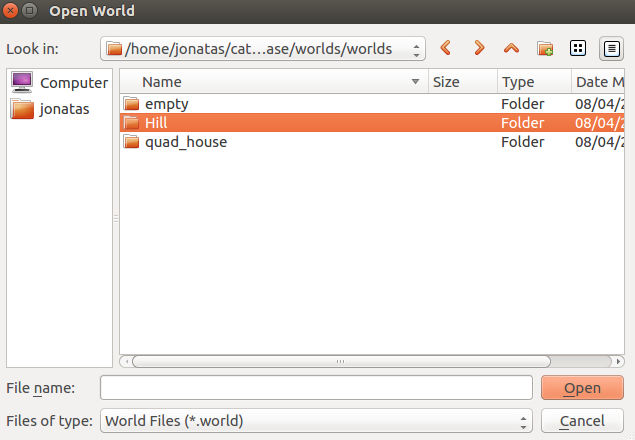
\includegraphics[width=250pt]{figuras/cenarioworld.png}
		\caption{UAV 4.0 Simulation.}
		\label{cenarioworld}
	\end{figure*}

	It's not necessary to select the UAV 4.0 model in the "Edit" option of the graphical interface top menu. The next step is to double-click the uri field in the main window of the graphical interface and in the top tab "Controller" select the control strategy "vant4Winf" and compile it using the "Compile" button.
	
	In the main window of the graphical interface the pose must be Position($0,0,0$) e Orientation($0,0,0$) as shown:
	
	
	\begin{figure*}[!ht]
		\centering
		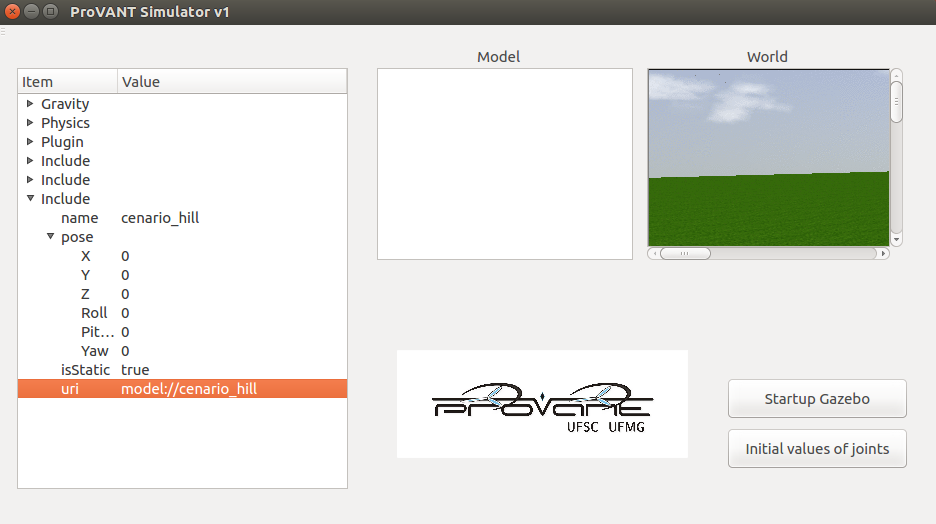
\includegraphics[width=250pt]{figuras/cenariogui.png}
		\caption{Main Window of the User Interface for UAV 4.0 with Scenario.}
		\label{cenariogui}
	\end{figure*}

	The simulation with the scenario is configured and the user should select the "Startup Gazebo" option in the main window of the user interface to launch it. The user can then select the Gazebo option "Step" to initialize the simulation.
	
	
	\begin{figure*}[!ht]
		\centering
		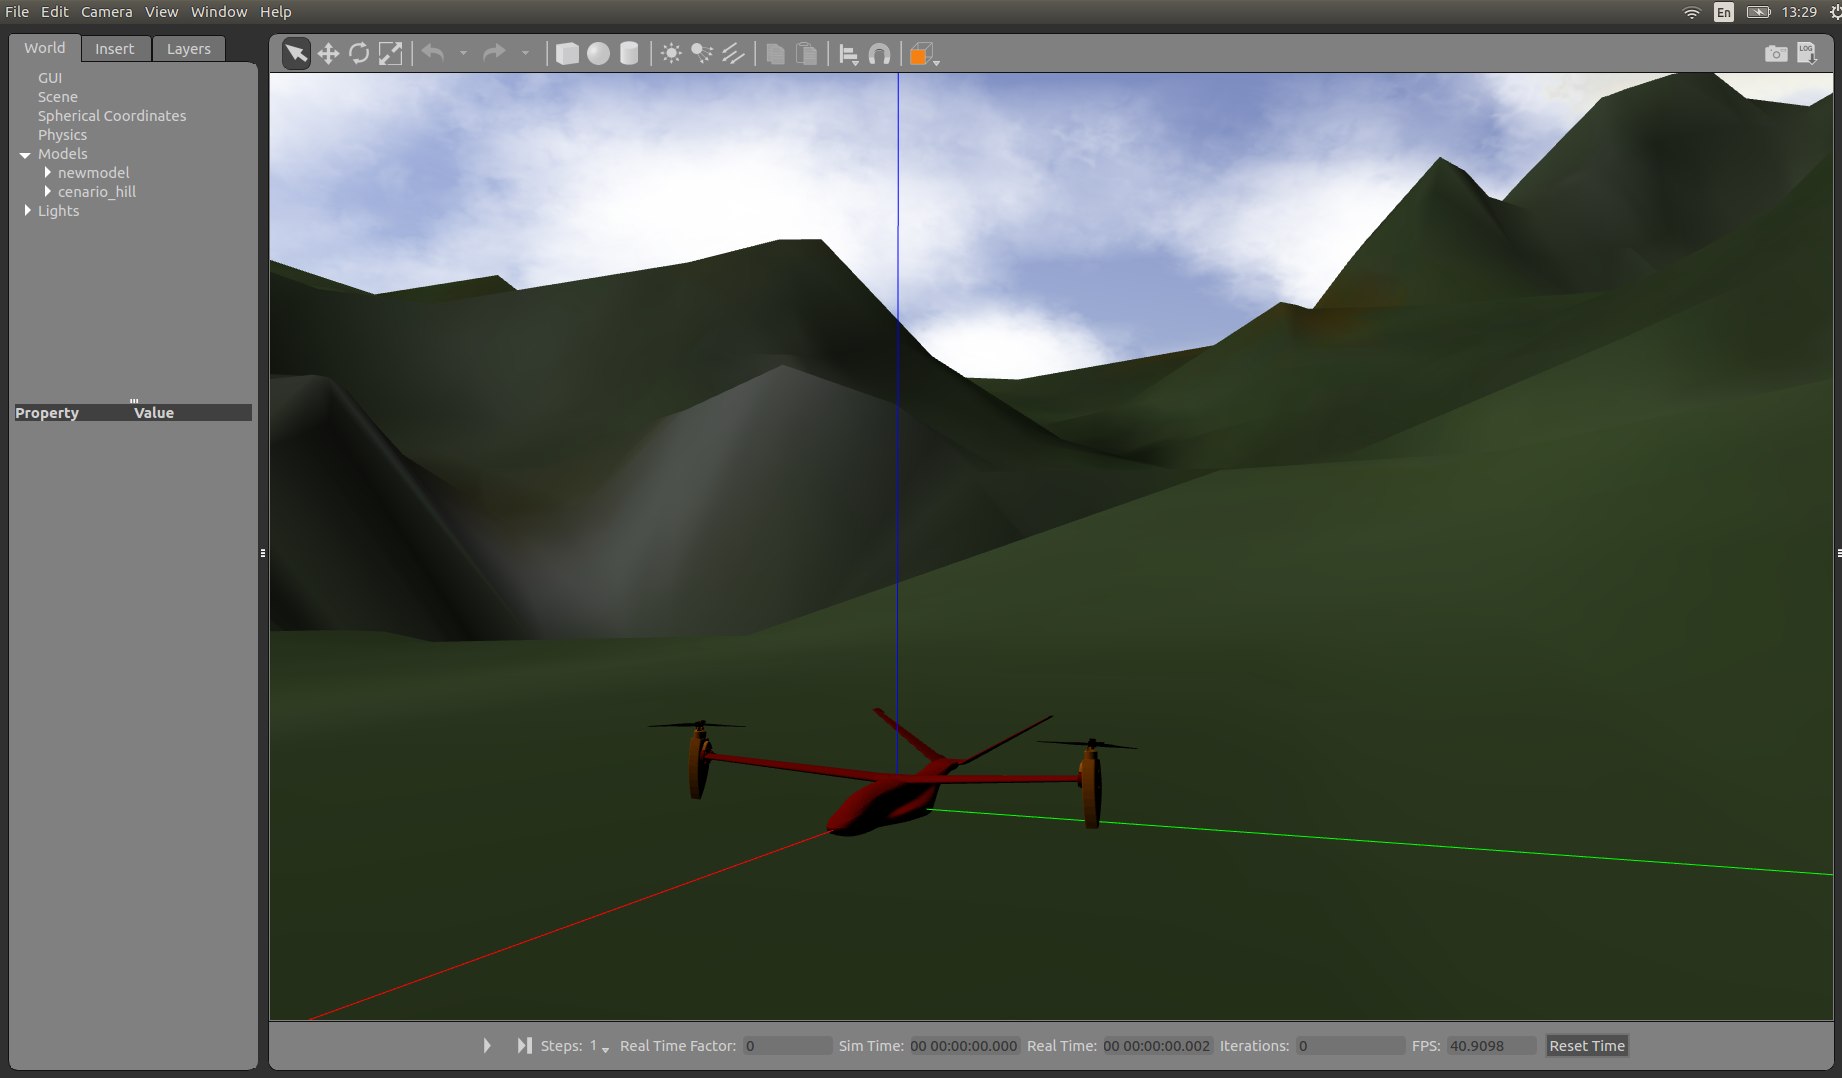
\includegraphics[width=250pt]{figuras/cenariosim.png}
		\caption{UAV 4.0 with Scenario Simulation.}
		\label{cenariosim}
	\end{figure*}
	
	\subsection{Visualizing UAV 4.0 Trajectory in Rviz}
	
	In order to visualize the UAV trajectory in Rviz the user first must follow the steps in the examples \textbf{VANT 4.0} or \textbf{VANT 4.0 com Cenário}. Then in a shell terminal the user can initialize Rviz to configure it.
	
	
	\begin{bashcode}
		$ rosrun rviz rviz
		\end{bashcode}

		The following screen must appear in Rviz
		
		
		\begin{figure*}[!ht]
			\centering
			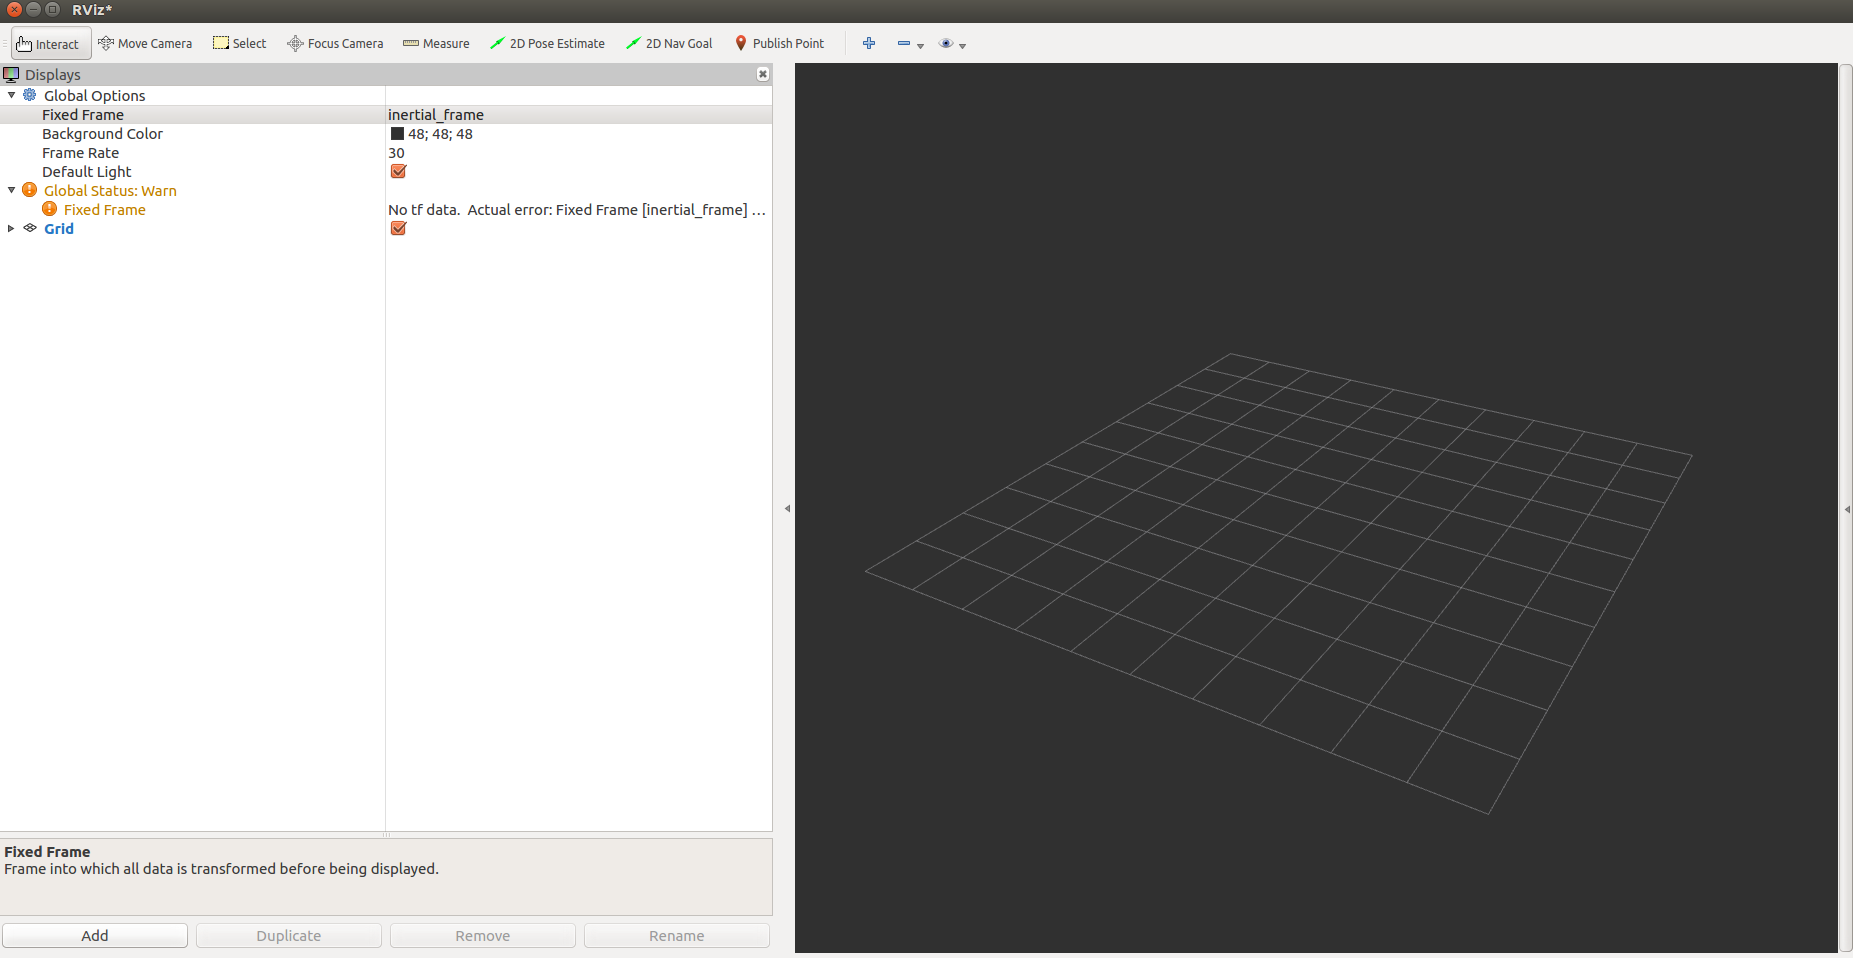
\includegraphics[width=450pt]{figuras/rvizconfig1.png}
			\caption{Rviz Main Window.}
			\label{rvizconfig1}
		\end{figure*}

		The option "\textit{fixed frame}"  should be configured to "\textit{inertial frame}". Next, select the \textit{display} "Path" available after selecting the "Add" button on the bottom Rviz menu.


		
		
		\begin{figure*}[!ht]
			\centering
			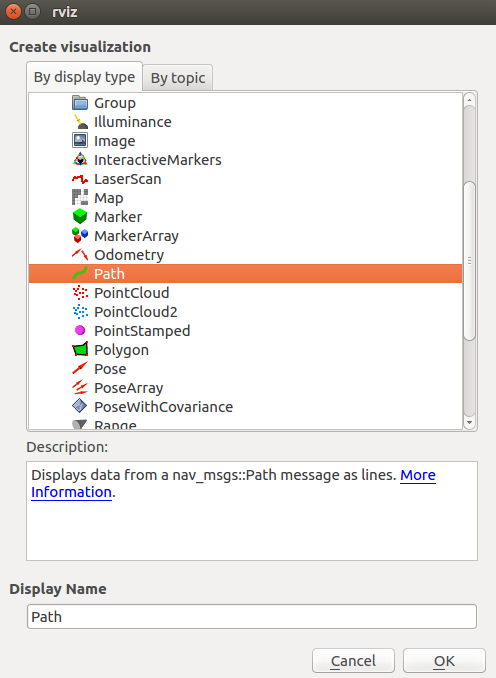
\includegraphics[width=150pt]{figuras/rvizconfig.png}
			\caption{Displays.}
			\label{rvizconfig}
		\end{figure*}
		
		To configure the "Path" \textit{display} three parameters should be configured: "topic","Buffer Length" and "Pose Style". 
		In "topic" the user should select the ros topic, \textit{/Path}, responsable to show the \textit{UAV real trajectory}. Higher values of "Buffer Length" allow the trajectory to stay visible for a long period of time, an empirical value of $12000$ proved to be enough for the simulation. For smaller values of "Buffer Length" the trajectory will be a trace behind the UAV. The last parameter, "Pose Style" should be selected as "Arrow". By modifying its subparameters is possible to configured the form of the trajectory according to the user's preference.
	
		
		
		\begin{figure*}[!ht]
			\centering
			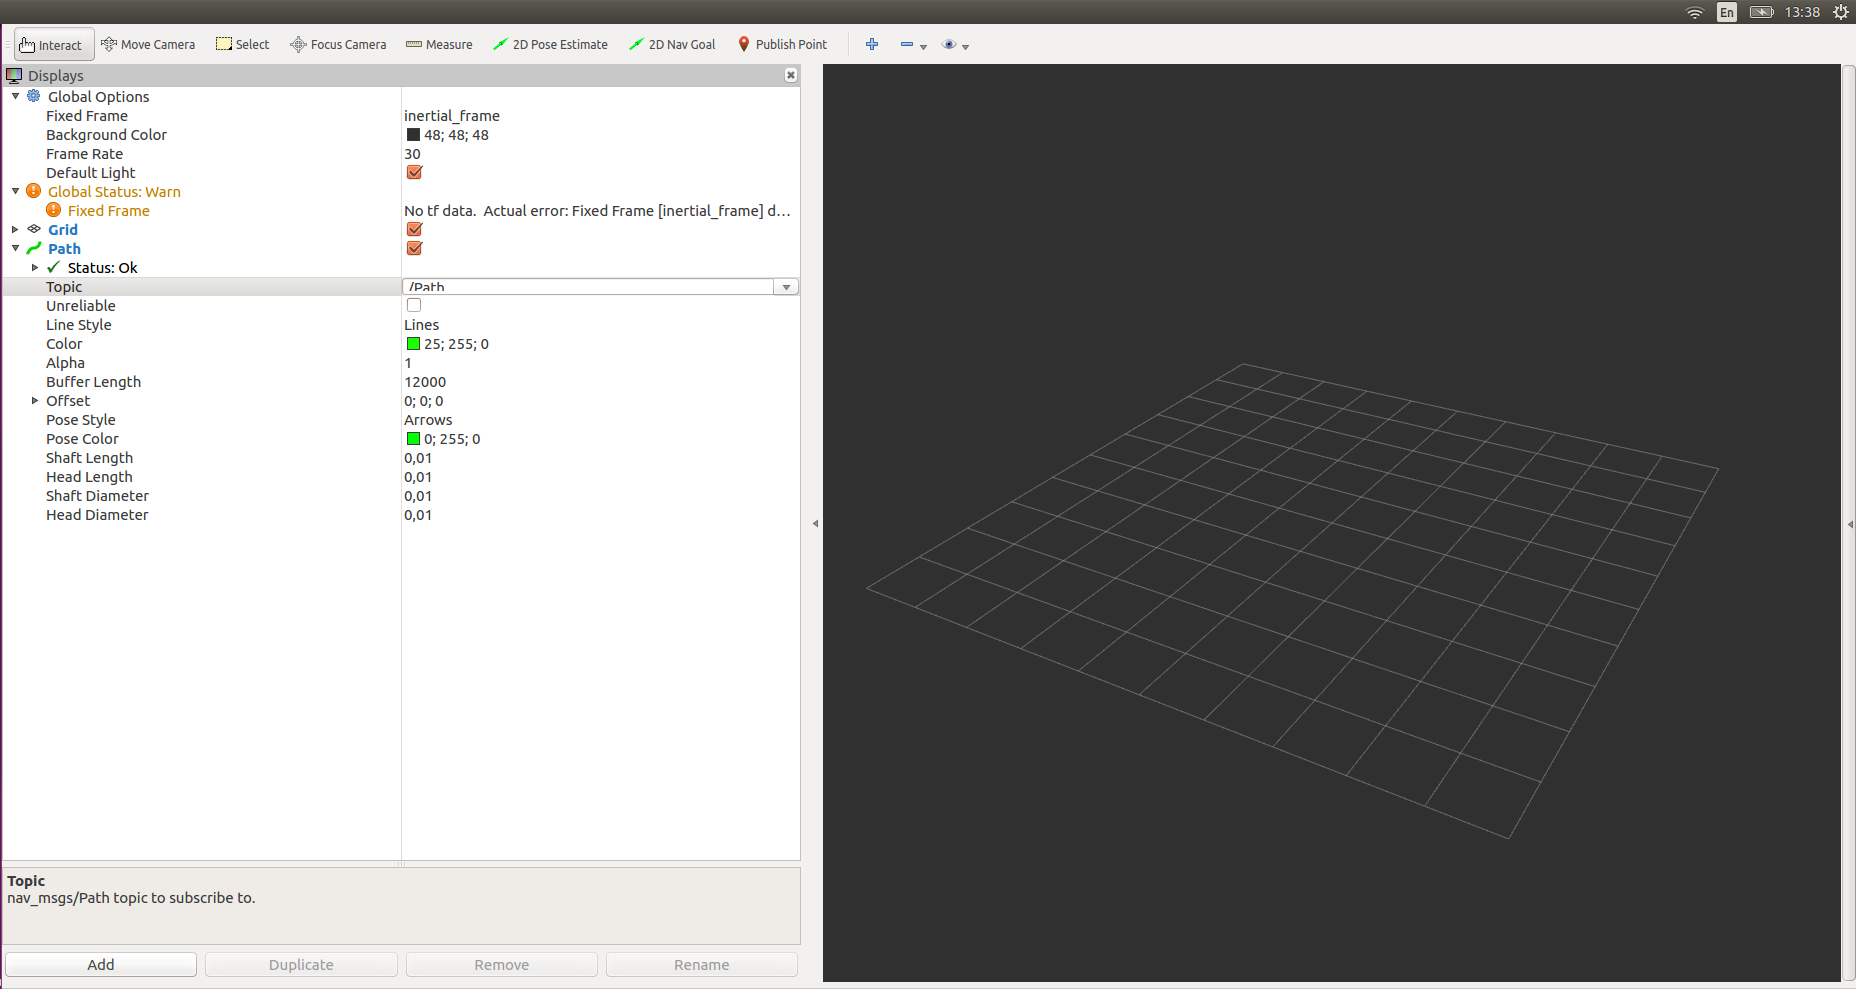
\includegraphics[width=450pt]{figuras/rvizconfig2.png}
			\caption{ Display \textit{/Path} Configuration.}
			\label{rvizconfig2}
		\end{figure*}
		
		Among the configurations the user can also modify the trajectory color.Next, the user should select another Path \textit{display} using the "Add" button. This time the \textit{display} should be configure to show the \textit{UAV reference trajectory} which can be done by setting the "topic" to \textit{/Path\_ref} and configuring the other parameters in the same way the \textit{UAV real trajectory} was configured. 
		
		Next the user should select the \textit{display} "Marker" by selecting the "Add" button. The only parameter to be configured here is the "Topic" that should be set to the ros topic responsible to make possible visualize the UAV in rviz, \textit{/marker}. Figure \ref{rvizmarker} ilustrates this process.
		
		\begin{figure*}[!ht]
			\centering
			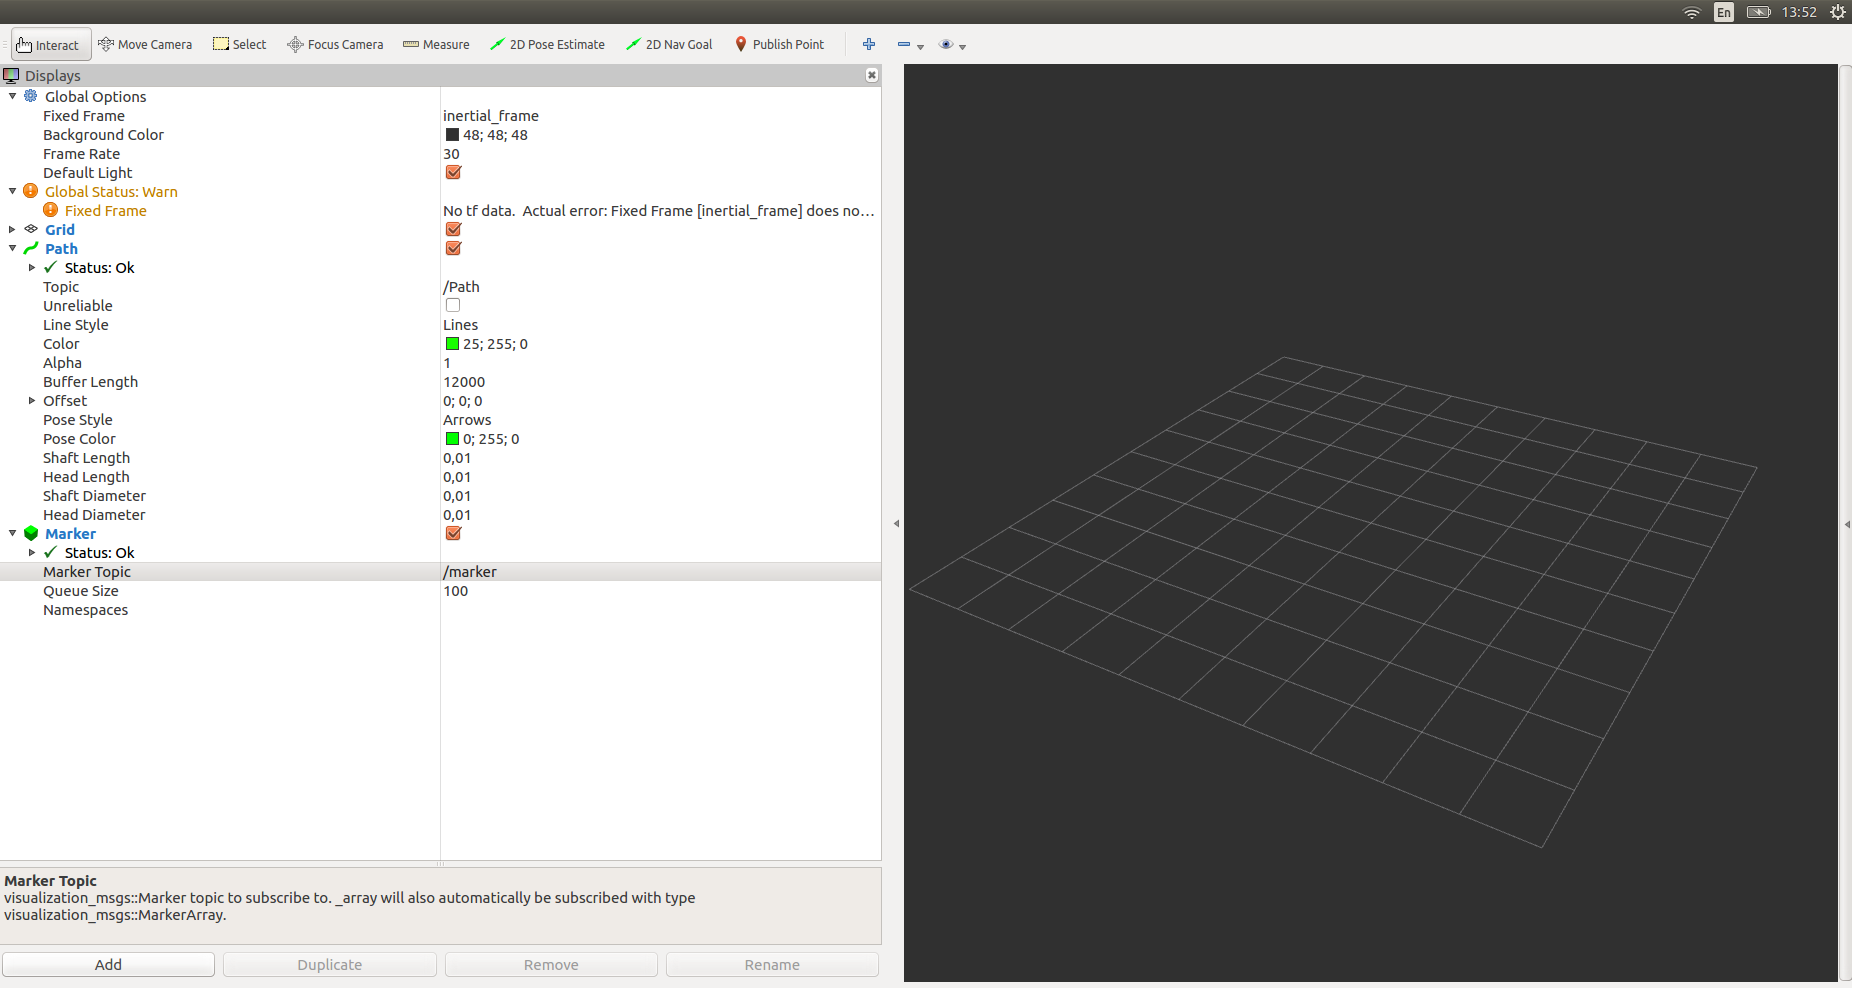
\includegraphics[width=350pt]{figuras/rvizmarker.png}
			\caption{\textit{/marker} Display Configuration.}
			\label{rvizmarker}
		\end{figure*}
		
		Rviz will then be configured and ready to be used. To visualize the UAV trajectory the user only needs to configure and start the simulation as showned by examples \textbf{UAV 4.0} or \textbf{UAV 4.0 with Scenario} according to the user's preference, then launch rviz. The trajectory should appear automaticaly in rviz as showned by figure \ref{rvizresult}.
		
		
		\begin{figure*}[!ht]
			\centering
			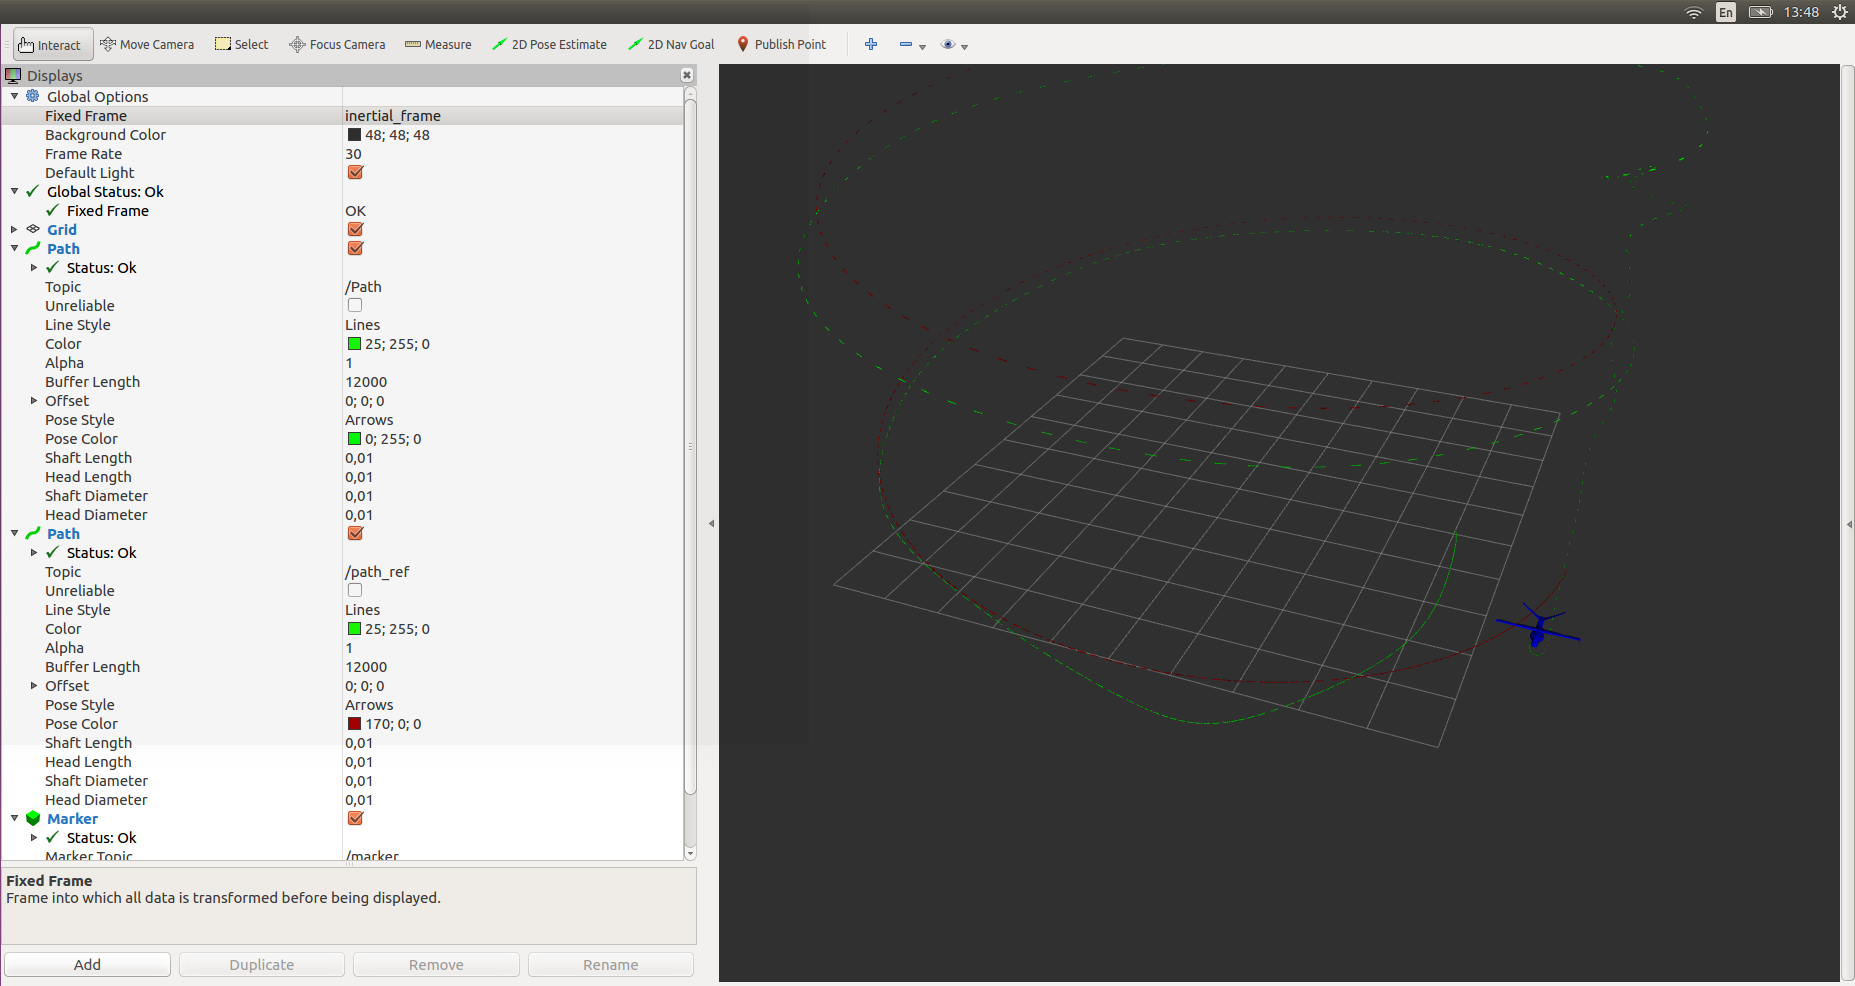
\includegraphics[width=350pt]{figuras/rvizresult.png}
			\caption{Rviz Trajectory.}
			\label{rvizresult}
		\end{figure*}
		
		%--------------------------------------------------------------------
		
		
		\subsection{Extra Funcionalities - Laser Sensor}
		
		The UAV 4.0 and Quadorotor both have a laser sensor for obstacle detection implemented. The parameters that control this funcionality are in the ".sdf" files that can be access using the path:
		
	\begin{bashcode}
$HOME/catkin_ws/src/ProVANT-Simulator/source/Database/models/vant_4_aerod/robot
		\end{bashcode}
			or for the Quadrotor
		\begin{bashcode}	$HOME/catkin_ws/src/ProVANT-Simulator/source/Database/models/quadcopter/robot
	\end{bashcode}
		
		In the ".sdf" file just bellow the link created for the sensor should be the description of the laser sensor. 
		
		\begin{minted}{xml}
		<sensor type="ray" name="laser">
		<pose>0 0 0 0 0 0</pose>
		<visualize>true</visualize>
		<update_rate>30</update_rate>
		<ray>
		<scan>
		<horizontal>
		<samples>40</samples>
		<resolution>1.0</resolution>
		<min_angle>-0.20</min_angle>
		<max_angle>0.1</max_angle>
		</horizontal>
		<vertical>
		<samples>40</samples>
		<resolution>1.0</resolution>
		<min_angle>-0.20</min_angle>
		<max_angle>0.1</max_angle>
		</vertical>
		</scan>
		<range>
		<min>0.01</min>
		<max>2.5</max>
		<resolution>0.02</resolution>
		</range>
		</ray>
		
		<plugin filename="libgazebo_ros_range.so" name="gazebo_ros_range">
		<gaussianNoise>0.005</gaussianNoise>
		<alwaysOn>true</alwaysOn>
		<updateRate>5</updateRate>
		<topicName>/sensor/laser</topicName>
		<frameName>laser_link</frameName>
		<visualize>true</visualize>
		<radiation>infrared</radiation>
		<fov>0.02</fov>
		</plugin>
		</sensor>
		\end{minted}
		Bellow, some important parameters the user can modify are listed.
		\begin{itemize}
			\setlength{\itemsep}{1pt}
			\setlength{\parskip}{0pt}
			\setlength{\parsep}{0pt}
			\item[-] \textcolor{blue}{<visualize></visualize>}: define if the laser beams will be visible in Gazebo;
			\item[-] \textcolor{blue}{<horizontal></horizontal>}: define parameters for horizontal laser beams.  
			\item[-] \textcolor{blue}{<vertical></vertical>}:define parameters for vertical laser beams. 
			\item[-] \textcolor{blue}{<samples></samples>}: define the number of laser beams. 
			\item[-] \textcolor{blue}{<resolution></resolution>}:\url{http://sdformat.org/spec?ver=1.6&elem=sensor#horizontal_resolution}. 
			\item[-] \textcolor{blue}{<min\_angle></min\_angle>}: define the minimum angle in radians. 
			\item[-] \textcolor{blue}{<max\_angle></max\_angle>}: define the maximum angle in radians. 
			\item[-] \textcolor{blue}{<range></range>}: define properties related to the range of the laser beam. 
			\item[-] \textcolor{blue}{<min></min>}: minimum range for the laser beam. 
			\item[-] \textcolor{blue}{<max></max>}: maximum range for the laser beam.
			\item[-] \textcolor{blue}{<topicName></topicName>}: name of the ros topic where the readings of the laser will be published.  
		\end{itemize}\normalsize
		The user can check the laser readings by typing the ros command bellow:
		\begin{bashcode}
			rostopic echo /sensor/laser
		\end{bashcode}
		
		\begin{figure*}[!ht]
			\centering
			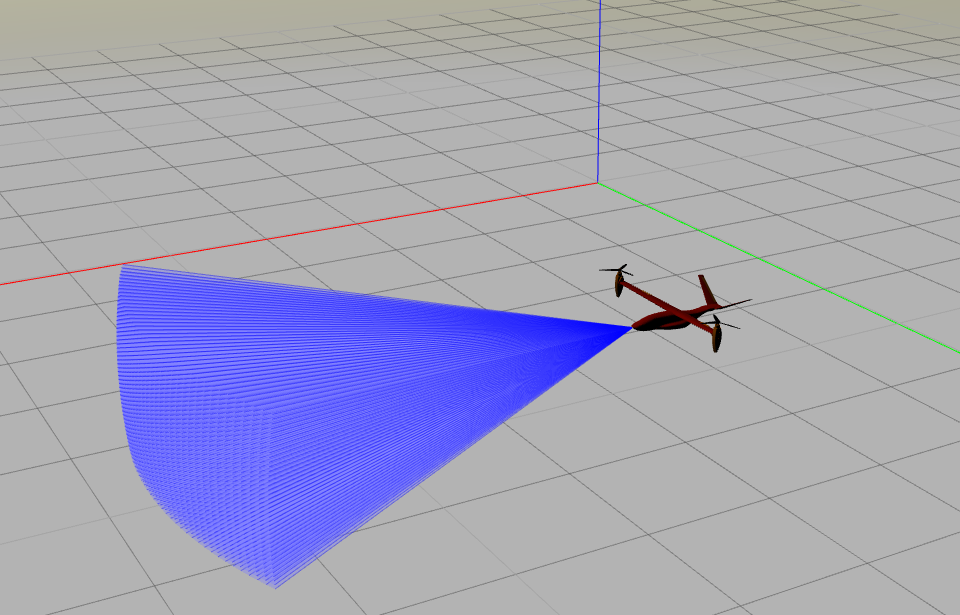
\includegraphics[width=250pt]{figuras/v4laser.png}
			\caption{UAV 4.0 Laser Sensor.}
			\label{v4laser}
		\end{figure*}
		
		\begin{figure*}[!ht]
			\centering
			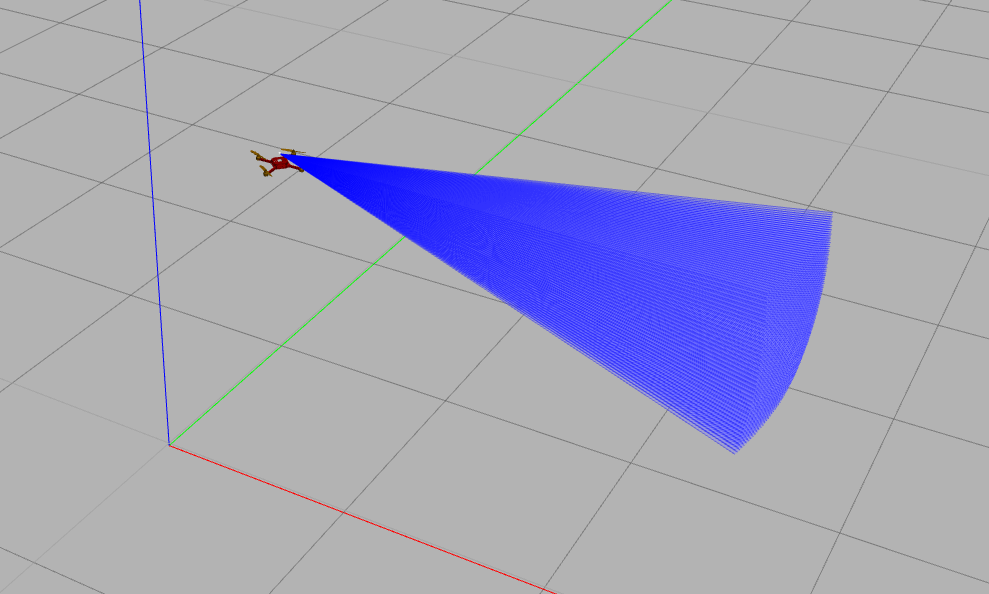
\includegraphics[width=250pt]{figuras/quadlaser.png}
			\caption{Quadrotor Laser Sensor.}
			\label{quadlaser}
		\end{figure*}
		
		
		
		%---------------------------------------------------------------------
		
		\subsection{Extra Funcionalities - First Person View}
		
		The UAV 4.0 and Quadrotor also have the first person view funcionality. This funcionality was implemented using a gazebo camera and allows the use to visualize the trajectory from the UAV perpective. The parameters that control this funcionality are in the UAV's ."sdf" files in the path:

		\begin{bashcode}	$HOME/catkin_ws/src/ProVANT-Simulator/source/Database/models/vant_4_aerod/robot
			\end{bashcode}
			or for the Quadrotor
			\begin{bashcode}	$HOME/catkin_ws/src/ProVANT-Simulator/source/Database/models/quadcopter/robot
		\end{bashcode}
	
	In the ".sdf" file just bellow the link created for the camera should be the description of the camera sensor.
		\begin{minted}{xml}
		<sensor name="camera" type="depth">
		<camera>
		<horizontal_fov>1.047</horizontal_fov>
		<image>
		<width>320</width>
		<height>240</height>
		</image>
		<clip>
		<near>0.1</near>
		<far>100</far>
		</clip>
		</camera>
		<always_on>1</always_on>
		<update_rate>30</update_rate>
		<visualize>true</visualize>
		<plugin name="camera_plugin" filename="libgazebo_ros_openni_kinect.so">
		<baseline>0.2</baseline>
		<alwaysOn>true</alwaysOn>
		<!-- Keep this zero, update_rate in the parent <sensor> tag
		will control the frame rate. -->
		<updateRate>0.0</updateRate>
		<cameraName>camera_ir</cameraName>
		<imageTopicName>/camera/color/image_raw</imageTopicName>
		<cameraInfoTopicName>/camera/color/camera_info</cameraInfoTopicName>
		<depthImageTopicName>/camera/depth/image_raw</depthImageTopicName>
		<depthImageCameraInfoTopicName>/camera/depth/camera_info</depthImageCameraInfoTopicName>
		<pointCloudTopicName>/camera/depth/points</pointCloudTopicName>
		<frameName>camera_link</frameName>
		<pointCloudCutoff>0.5</pointCloudCutoff>
		<pointCloudCutoffMax>3.0</pointCloudCutoffMax>
		<distortionK1>0</distortionK1>
		<distortionK2>0</distortionK2>
		<distortionK3>0</distortionK3>
		<distortionT1>0</distortionT1>
		<distortionT2>0</distortionT2>
		<CxPrime>0</CxPrime>
		<Cx>0</Cx>
		<Cy>0</Cy>
		<focalLength>0</focalLength>
		<hackBaseline>0</hackBaseline>
		</plugin>
		</sensor>
		\end{minted}
		\centerline{Code: Camera functionality in "model.sdf" file}
		
		This sensor can works as a normal camera or as a depth camera where obstacles can be identify in rviz using the \textit{PointCloud2} rviz display.
		The first thing the user should do afeter launching Rviz is to change the option "Fixed Frame" to the option in the ".sdf" tag \textcolor{blue}{<frameName></frameName>}, "camera\_link", then add the rviz \textit{display} camera.
		
		\begin{figure*}[!ht]
			\centering
			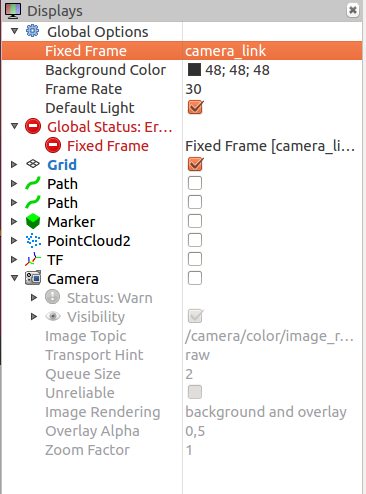
\includegraphics[width=150pt]{figuras/camrviz.png}
			\caption{Camera \textit{Display} Configuration }
			\label{camrviz}
		\end{figure*}
		
		The rviz "topic" parameter shoul be set to the ros topic name defined in the ".sdf" file in the \textcolor{blue}{<imageTopicName></imageTopicName>} tag.
		When a simulation with the UAV 4.0 or Quadrotor is launched will be possible to use rviz to visualize the trajectory from the UAV perspective. 
		
		
		\begin{figure*}[!ht]
			\centering
			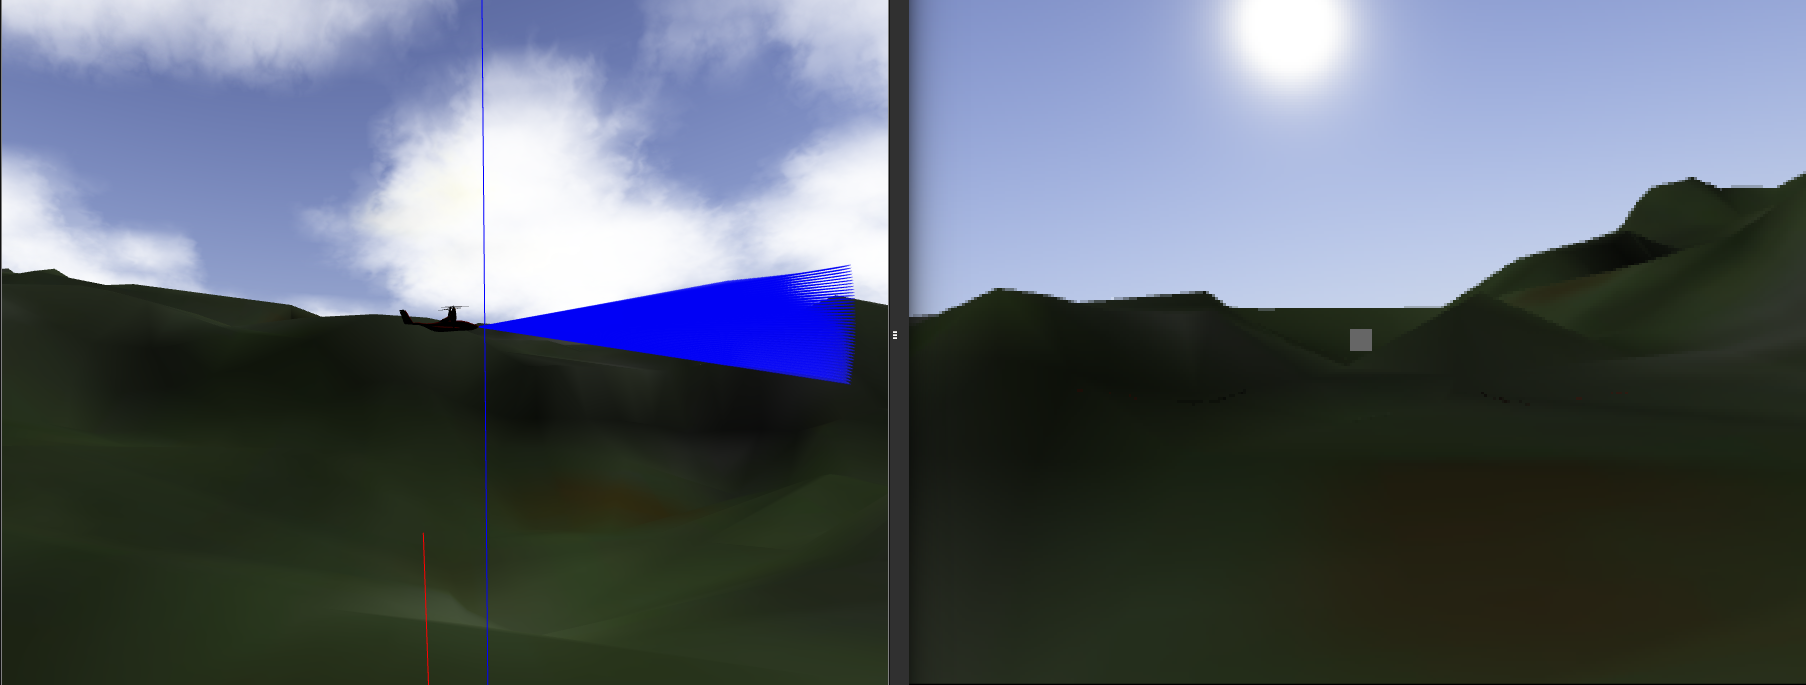
\includegraphics[width=450pt]{figuras/camerav4.png}
			\caption{UAV 4.0 First Person View.}
			\label{v4camera}
		\end{figure*}
		
		\begin{figure*}[!ht]
			\centering
			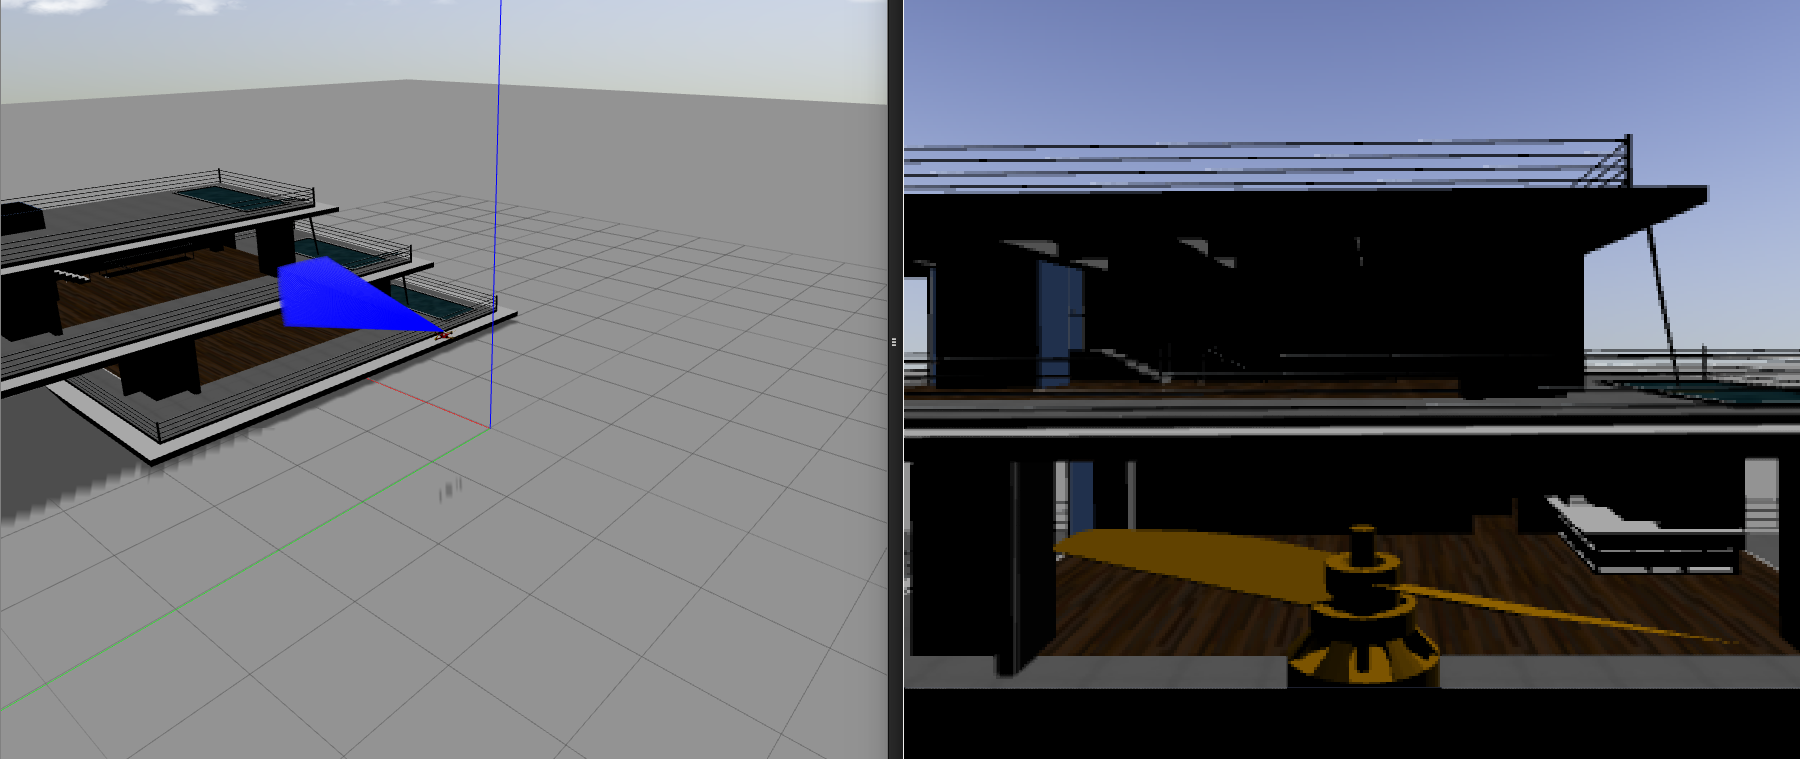
\includegraphics[width=450pt]{figuras/quadcam.png}
			\caption{Quadrotor First Person View.}
			\label{quadamera}
		\end{figure*}





%------------------------------------------------------------------------